%Chapter 1
\chapter{Introduction and background}  %J.H Marais, C.J.R. Kriel
\pagenumbering{arabic} 
\setcounter{page}{1}
\vspace{38em}

\hrulefill
\\
\enquote*{\textit{Your ideas are like diamonds. Without the refining process they are just rock. But cutting away impurities, they become priceless.}} - Paul Kearly\\
\newpage


\section{Preamble}

\section{Background on deep level mining}

\subsection{Mining profitability}
Background on rising mining costs (energy, wages, etc), falling ore grades and Eskom tariffs.\cite{neingo2016trends}
%\begin{figure}
%	\centering
%	% GNUPLOT: LaTeX picture with Postscript
\begingroup
  \makeatletter
  \providecommand\color[2][]{%
    \GenericError{(gnuplot) \space\space\space\@spaces}{%
      Package color not loaded in conjunction with
      terminal option `colourtext'%
    }{See the gnuplot documentation for explanation.%
    }{Either use 'blacktext' in gnuplot or load the package
      color.sty in LaTeX.}%
    \renewcommand\color[2][]{}%
  }%
  \providecommand\includegraphics[2][]{%
    \GenericError{(gnuplot) \space\space\space\@spaces}{%
      Package graphicx or graphics not loaded%
    }{See the gnuplot documentation for explanation.%
    }{The gnuplot epslatex terminal needs graphicx.sty or graphics.sty.}%
    \renewcommand\includegraphics[2][]{}%
  }%
  \providecommand\rotatebox[2]{#2}%
  \@ifundefined{ifGPcolor}{%
    \newif\ifGPcolor
    \GPcolortrue
  }{}%
  \@ifundefined{ifGPblacktext}{%
    \newif\ifGPblacktext
    \GPblacktextfalse
  }{}%
  % define a \g@addto@macro without @ in the name:
  \let\gplgaddtomacro\g@addto@macro
  % define empty templates for all commands taking text:
  \gdef\gplbacktext{}%
  \gdef\gplfronttext{}%
  \makeatother
  \ifGPblacktext
    % no textcolor at all
    \def\colorrgb#1{}%
    \def\colorgray#1{}%
  \else
    % gray or color?
    \ifGPcolor
      \def\colorrgb#1{\color[rgb]{#1}}%
      \def\colorgray#1{\color[gray]{#1}}%
      \expandafter\def\csname LTw\endcsname{\color{white}}%
      \expandafter\def\csname LTb\endcsname{\color{black}}%
      \expandafter\def\csname LTa\endcsname{\color{black}}%
      \expandafter\def\csname LT0\endcsname{\color[rgb]{1,0,0}}%
      \expandafter\def\csname LT1\endcsname{\color[rgb]{0,1,0}}%
      \expandafter\def\csname LT2\endcsname{\color[rgb]{0,0,1}}%
      \expandafter\def\csname LT3\endcsname{\color[rgb]{1,0,1}}%
      \expandafter\def\csname LT4\endcsname{\color[rgb]{0,1,1}}%
      \expandafter\def\csname LT5\endcsname{\color[rgb]{1,1,0}}%
      \expandafter\def\csname LT6\endcsname{\color[rgb]{0,0,0}}%
      \expandafter\def\csname LT7\endcsname{\color[rgb]{1,0.3,0}}%
      \expandafter\def\csname LT8\endcsname{\color[rgb]{0.5,0.5,0.5}}%
    \else
      % gray
      \def\colorrgb#1{\color{black}}%
      \def\colorgray#1{\color[gray]{#1}}%
      \expandafter\def\csname LTw\endcsname{\color{white}}%
      \expandafter\def\csname LTb\endcsname{\color{black}}%
      \expandafter\def\csname LTa\endcsname{\color{black}}%
      \expandafter\def\csname LT0\endcsname{\color{black}}%
      \expandafter\def\csname LT1\endcsname{\color{black}}%
      \expandafter\def\csname LT2\endcsname{\color{black}}%
      \expandafter\def\csname LT3\endcsname{\color{black}}%
      \expandafter\def\csname LT4\endcsname{\color{black}}%
      \expandafter\def\csname LT5\endcsname{\color{black}}%
      \expandafter\def\csname LT6\endcsname{\color{black}}%
      \expandafter\def\csname LT7\endcsname{\color{black}}%
      \expandafter\def\csname LT8\endcsname{\color{black}}%
    \fi
  \fi
    \setlength{\unitlength}{0.0500bp}%
    \ifx\gptboxheight\undefined%
      \newlength{\gptboxheight}%
      \newlength{\gptboxwidth}%
      \newsavebox{\gptboxtext}%
    \fi%
    \setlength{\fboxrule}{0.5pt}%
    \setlength{\fboxsep}{1pt}%
\begin{picture}(7200.00,5040.00)%
    \gplgaddtomacro\gplbacktext{%
      \colorrgb{0.50,0.50,0.50}%
      \put(1078,924){\makebox(0,0)[r]{\strut{}$8500$}}%
      \colorrgb{0.50,0.50,0.50}%
      \put(1078,1269){\makebox(0,0)[r]{\strut{}$9000$}}%
      \colorrgb{0.50,0.50,0.50}%
      \put(1078,1615){\makebox(0,0)[r]{\strut{}$9500$}}%
      \colorrgb{0.50,0.50,0.50}%
      \put(1078,1960){\makebox(0,0)[r]{\strut{}$10000$}}%
      \colorrgb{0.50,0.50,0.50}%
      \put(1078,2306){\makebox(0,0)[r]{\strut{}$10500$}}%
      \colorrgb{0.50,0.50,0.50}%
      \put(1078,2651){\makebox(0,0)[r]{\strut{}$11000$}}%
      \colorrgb{0.50,0.50,0.50}%
      \put(1078,2997){\makebox(0,0)[r]{\strut{}$11500$}}%
      \colorrgb{0.50,0.50,0.50}%
      \put(1078,3342){\makebox(0,0)[r]{\strut{}$12000$}}%
      \colorrgb{0.50,0.50,0.50}%
      \put(1078,3688){\makebox(0,0)[r]{\strut{}$12500$}}%
      \colorrgb{0.50,0.50,0.50}%
      \put(1078,4033){\makebox(0,0)[r]{\strut{}$13000$}}%
      \colorrgb{0.50,0.50,0.50}%
      \put(1078,4379){\makebox(0,0)[r]{\strut{}$13500$}}%
      \colorrgb{0.50,0.50,0.50}%
      \put(1210,704){\makebox(0,0){\strut{}$2011$}}%
      \colorrgb{0.50,0.50,0.50}%
      \put(2329,704){\makebox(0,0){\strut{}$2012$}}%
      \colorrgb{0.50,0.50,0.50}%
      \put(3447,704){\makebox(0,0){\strut{}$2013$}}%
      \colorrgb{0.50,0.50,0.50}%
      \put(4566,704){\makebox(0,0){\strut{}$2014$}}%
      \colorrgb{0.50,0.50,0.50}%
      \put(5684,704){\makebox(0,0){\strut{}$2015$}}%
      \colorrgb{0.50,0.50,0.50}%
      \put(6803,704){\makebox(0,0){\strut{}$2016$}}%
    }%
    \gplgaddtomacro\gplfronttext{%
      \csname LTb\endcsname%
      \put(176,2651){\rotatebox{-270}{\makebox(0,0){\strut{}y axis label}}}%
      \put(4006,374){\makebox(0,0){\strut{}x axis label}}%
      \put(4006,4709){\makebox(0,0){\strut{}Title}}%
      \csname LTb\endcsname%
      \put(4701,173){\makebox(0,0)[r]{\strut{}'HarmonyCost.dat'}}%
    }%
    \gplbacktext
    \put(0,0){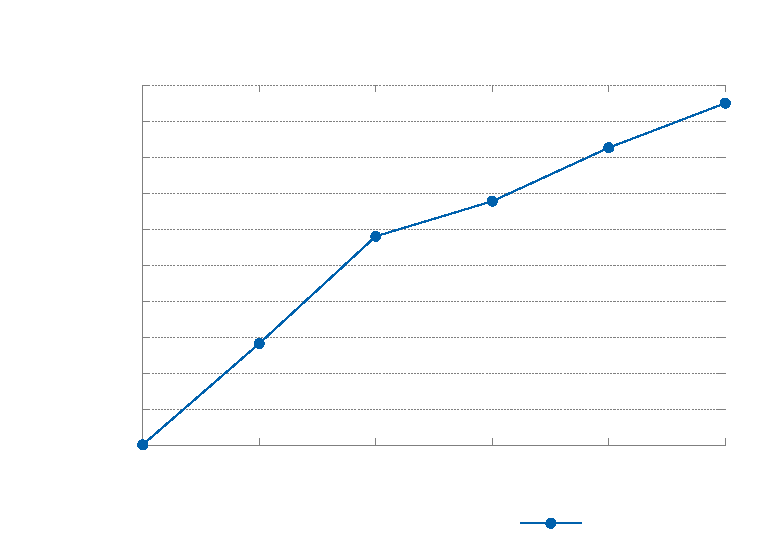
\includegraphics{Graphs/introduction}}%
    \gplfronttext
  \end{picture}%
\endgroup

%\end{figure} 


\subsection{Mining systems and energy}
Focus an mine electrical energy users. Compressed air and its inefficiencies
\subsection{Need to improve service delivery}
\section{Mining compressed air}
The supply of compressed air is highly energy demanding and costly process \cite{padachi2009energy}.  According to *** energy related to the production of compressed air made up approximately x\% of total industrial energy demand ***need a recent source for this***.
However, 
\subsection{Compressed air in operation}
	Due to their reliability, versatilely and ease of use, South African gold and platinum mines have installed extensive air networks. These systems can have compressors with capacities of up to 15 \gls{mw}\cite{Marais2012PhD}.\par
	Compressed air is utilised for a variety of applications in the mining industry.
	
	A study by  Bester \textit{et al.} showed that between 2002 and 2013 compressed air and energy consumption had steadily increased as shown in \ref{fig: Compressed energy and air flow per ton}. The increase in consumption is a result of a reduction in air pressure at the mining stopes. Measurements indicated that the pressure was as low as 300 \gls{kpa}. This would have an effect the efficiency of the rock drills. Historically, before 2002, pressure was maintained above 500 \gls{kpa} at the stopes.  It was concluded that the lower pressure was the cause of the slower drilling rate.\cite{bester2013effect} \par
	
	\begin{figure}
		\centering
		% GNUPLOT: LaTeX picture with Postscript
\begingroup
\makeatletter
\providecommand\color[2][]{%
	\GenericError{(gnuplot) \space\space\space\@spaces}{%
		Package color not loaded in conjunction with
		terminal option `colourtext'%
	}{See the gnuplot documentation for explanation.%
	}{Either use 'blacktext' in gnuplot or load the package
		color.sty in LaTeX.}%
	\renewcommand\color[2][]{}%
}%
\providecommand\includegraphics[2][]{%
	\GenericError{(gnuplot) \space\space\space\@spaces}{%
		Package graphicx or graphics not loaded%
	}{See the gnuplot documentation for explanation.%
	}{The gnuplot epslatex terminal needs graphicx.sty or graphics.sty.}%
	\renewcommand\includegraphics[2][]{}%
}%
\providecommand\rotatebox[2]{#2}%
\@ifundefined{ifGPcolor}{%
	\newif\ifGPcolor
	\GPcolortrue
}{}%
\@ifundefined{ifGPblacktext}{%
	\newif\ifGPblacktext
	\GPblacktextfalse
}{}%
% define a \g@addto@macro without @ in the name:
\let\gplgaddtomacro\g@addto@macro
% define empty templates for all commands taking text:
\gdef\gplbacktext{}%
\gdef\gplfronttext{}%
\makeatother
\ifGPblacktext
% no textcolor at all
\def\colorrgb#1{}%
\def\colorgray#1{}%
\else
% gray or color?
\ifGPcolor
\def\colorrgb#1{\color[rgb]{#1}}%
\def\colorgray#1{\color[gray]{#1}}%
\expandafter\def\csname LTw\endcsname{\color{white}}%
\expandafter\def\csname LTb\endcsname{\color{black}}%
\expandafter\def\csname LTa\endcsname{\color{black}}%
\expandafter\def\csname LT0\endcsname{\color[rgb]{1,0,0}}%
\expandafter\def\csname LT1\endcsname{\color[rgb]{0,1,0}}%
\expandafter\def\csname LT2\endcsname{\color[rgb]{0,0,1}}%
\expandafter\def\csname LT3\endcsname{\color[rgb]{1,0,1}}%
\expandafter\def\csname LT4\endcsname{\color[rgb]{0,1,1}}%
\expandafter\def\csname LT5\endcsname{\color[rgb]{1,1,0}}%
\expandafter\def\csname LT6\endcsname{\color[rgb]{0,0,0}}%
\expandafter\def\csname LT7\endcsname{\color[rgb]{1,0.3,0}}%
\expandafter\def\csname LT8\endcsname{\color[rgb]{0.5,0.5,0.5}}%
\else
% gray
\def\colorrgb#1{\color{black}}%
\def\colorgray#1{\color[gray]{#1}}%
\expandafter\def\csname LTw\endcsname{\color{white}}%
\expandafter\def\csname LTb\endcsname{\color{black}}%
\expandafter\def\csname LTa\endcsname{\color{black}}%
\expandafter\def\csname LT0\endcsname{\color{black}}%
\expandafter\def\csname LT1\endcsname{\color{black}}%
\expandafter\def\csname LT2\endcsname{\color{black}}%
\expandafter\def\csname LT3\endcsname{\color{black}}%
\expandafter\def\csname LT4\endcsname{\color{black}}%
\expandafter\def\csname LT5\endcsname{\color{black}}%
\expandafter\def\csname LT6\endcsname{\color{black}}%
\expandafter\def\csname LT7\endcsname{\color{black}}%
\expandafter\def\csname LT8\endcsname{\color{black}}%
\fi
\fi
\setlength{\unitlength}{0.0500bp}%
\ifx\gptboxheight\undefined%
\newlength{\gptboxheight}%
\newlength{\gptboxwidth}%
\newsavebox{\gptboxtext}%
\fi%
\setlength{\fboxrule}{0.5pt}%
\setlength{\fboxsep}{1pt}%
\begin{picture}(9360.00,4032.00)%
\gplgaddtomacro\gplbacktext{%
	\colorrgb{0.42,0.42,0.42}%
	\put(682,924){\makebox(0,0)[r]{\strut{}$0$}}%
	\colorrgb{0.42,0.42,0.42}%
	\put(682,1230){\makebox(0,0)[r]{\strut{}$5$}}%
	\colorrgb{0.42,0.42,0.42}%
	\put(682,1536){\makebox(0,0)[r]{\strut{}$10$}}%
	\colorrgb{0.42,0.42,0.42}%
	\put(682,1842){\makebox(0,0)[r]{\strut{}$15$}}%
	\colorrgb{0.42,0.42,0.42}%
	\put(682,2148){\makebox(0,0)[r]{\strut{}$20$}}%
	\colorrgb{0.42,0.42,0.42}%
	\put(682,2453){\makebox(0,0)[r]{\strut{}$25$}}%
	\colorrgb{0.42,0.42,0.42}%
	\put(682,2759){\makebox(0,0)[r]{\strut{}$30$}}%
	\colorrgb{0.42,0.42,0.42}%
	\put(682,3065){\makebox(0,0)[r]{\strut{}$35$}}%
	\colorrgb{0.42,0.42,0.42}%
	\put(682,3371){\makebox(0,0)[r]{\strut{}$40$}}%
	\colorrgb{0.42,0.42,0.42}%
	\put(814,704){\makebox(0,0){\strut{}$2002$}}%
	\colorrgb{0.42,0.42,0.42}%
	\put(2025,704){\makebox(0,0){\strut{}$2004$}}%
	\colorrgb{0.42,0.42,0.42}%
	\put(3237,704){\makebox(0,0){\strut{}$2006$}}%
	\colorrgb{0.42,0.42,0.42}%
	\put(4448,704){\makebox(0,0){\strut{}$2008$}}%
	\colorrgb{0.42,0.42,0.42}%
	\put(5659,704){\makebox(0,0){\strut{}$2010$}}%
	\colorrgb{0.42,0.42,0.42}%
	\put(6871,704){\makebox(0,0){\strut{}$2012$}}%
	\colorrgb{0.42,0.42,0.42}%
	\put(8082,704){\makebox(0,0){\strut{}$2014$}}%
	\colorrgb{0.42,0.42,0.42}%
	\put(8214,924){\makebox(0,0)[l]{\strut{}$0$}}%
	\colorrgb{0.42,0.42,0.42}%
	\put(8214,1230){\makebox(0,0)[l]{\strut{}$50$}}%
	\colorrgb{0.42,0.42,0.42}%
	\put(8214,1536){\makebox(0,0)[l]{\strut{}$100$}}%
	\colorrgb{0.42,0.42,0.42}%
	\put(8214,1842){\makebox(0,0)[l]{\strut{}$150$}}%
	\colorrgb{0.42,0.42,0.42}%
	\put(8214,2148){\makebox(0,0)[l]{\strut{}$200$}}%
	\colorrgb{0.42,0.42,0.42}%
	\put(8214,2453){\makebox(0,0)[l]{\strut{}$250$}}%
	\colorrgb{0.42,0.42,0.42}%
	\put(8214,2759){\makebox(0,0)[l]{\strut{}$300$}}%
	\colorrgb{0.42,0.42,0.42}%
	\put(8214,3065){\makebox(0,0)[l]{\strut{}$350$}}%
	\colorrgb{0.42,0.42,0.42}%
	\put(8214,3371){\makebox(0,0)[l]{\strut{}$400$}}%
}%
\gplgaddtomacro\gplfronttext{%
	\csname LTb\endcsname%
	\put(176,2147){\rotatebox{-270}{\makebox(0,0){\strut{}kWh/t}}}%
	\put(8851,2147){\rotatebox{-270}{\makebox(0,0){\strut{}$m^3$/t}}}%
	\put(4448,374){\makebox(0,0){\strut{}Year}}%
	\put(4448,3701){\makebox(0,0){\strut{}Compressed air energy and volume consumed per Tonne}}%
	\csname LTb\endcsname%
	\put(3593,173){\makebox(0,0)[r]{\strut{}Energy per Tonne (kWh/t)}}%
	\csname LTb\endcsname%
	\put(7352,173){\makebox(0,0)[r]{\strut{}Volume per Tonne ($m^3$/t)}}%
}%
\gplbacktext
\put(0,0){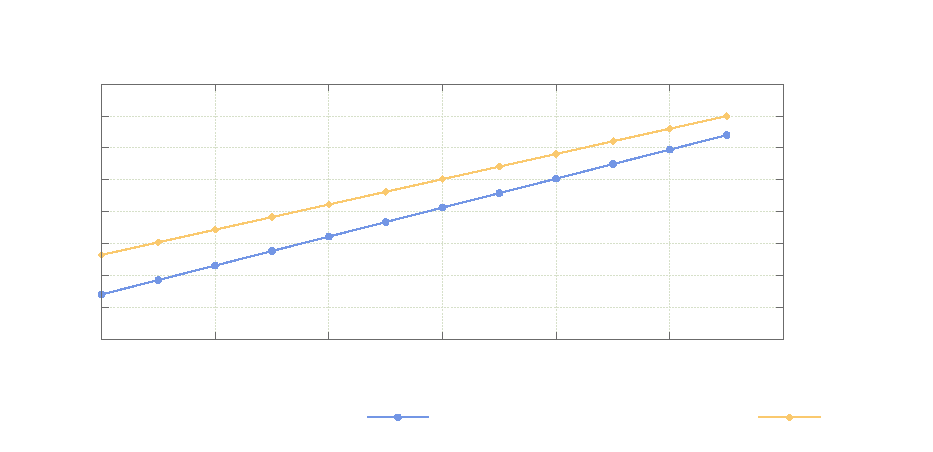
\includegraphics{Graphs/EVperT}}%
\gplfronttext
\end{picture}%
\endgroup
		\caption[The compressed air energy and flow per tonne of ore produced.]{The compressed air energy and flow per \gls{t} of ore produced, adopted from Bester \textit{et al.} \cite{bester2013effect}.}
		\label{fig: Compressed energy and air flow per ton}
	\end{figure}

	\subsection{Characteristic inefficiencies}
	\subsection{Inefficiency identification methods}
	\subsection{Instrumentation and measurements}
\section{Simulations in industry}

Continuous improvements in computing hardware has led to major advancement in software technology. Consequently the use of computational simulation has become an increasingly valuable tool for many industries.\cite{kocsis2003integration} \par 

 In \textit{ Handbook of simulation: principles, methodology, advances, applications, and practice} Banks discusses some of the advantages of the use of simulation in industry: \cite{banks1998handbook}:
\begin{itemize}
	\item The ability to test new policies, operating procedures and methods without causing a disruption to the actual system.
	\item Identify problems in complex systems by gathering insight in the interactions within the system.
	\item Simulation allows you to compress or expand time to investigate phenomena thoroughly.
	\item With simulation the limits and constraints within a system can be determined.
	\item Stimulation can help build consensus with regard to proposed designs or modifications.
\end{itemize}

\subsection{Thermal-hydraulic simulation}
\gls{ths} is the modelling and  computational analysis of Thermal-hydraulic
\paragraph{KY Pipe}
Ky pipe background. \cite{Wood1993KYPipe}
\paragraph{Simulation toolbox}
STB background.
\section{Problem statement and objectives}
\section{Dissertation overview}